% !TeX spellcheck = en_US
\addscenariosection{1}{Clash Scenario}{The Hunt}{\images/slayer.png}

\begin{multicols*}{2}

\textbf{Author:} Mateusz ``MATMOT'' Motyka

\textbf{Source:} \href{https://boardgamegeek.com/filepage/277736/clash-scenario-the-hunt-v10}{BoardGameGeek}

\textit{The land quivers under the reign of the fearsome Dragon.
  The one who dares to slay this monstrous beast shall ascend to the throne, crowned as the rightful ruler of the shattered kingdom.
}

\subsection*{\MakeUppercase{Scenario Length}}
This Scenario is played over 14 Rounds.

\subsection*{\MakeUppercase{Player Setup}}
\textbf{Player Count:} 2 or 3

\textbf{Starting Resources:} 15 \svg{gold}, 4 \svg{building_materials}, 2 \svg{valuables}

\textbf{Starting Income:} 10 \svg{gold}, 2 \svg{building_materials}, 1 \svg{valuables}

\textbf{Starting Units:}
\begin{itemize}
  \item A Pack of \svgunit{bronze} Units with the \textit{lowest} Recruitment cost
  \item A Few \svgunit{bronze} Units with the \textit{highest} Recruitment cost
\end{itemize}

\textbf{Town Buildings:} \svgunit{bronze} Dwelling, City Hall

\textbf{Map Tile Pool:} Each player takes 1 random Far (II--III) Map Tile

\subsection*{\MakeUppercase{Map Setup}}

Take the following Map Tiles and arrange them as shown in the Scenario map layout.

\textbf{For a 2-player Scenario:}
\begin{itemize}
  \item 2 × Starting (I) Map Tile
  \item 2 × Far (II--III) Map Tile
  \item 2 × Near (IV--V) Map Tile
  \item 1 × Center (VI--VII) Map Tile
\end{itemize}

\textbf{For a 3-player Scenario:}
\begin{itemize}
  \item 3 × Starting (I) Map Tile
  \item 3 × Far (II--III) Map Tile
  \item 3 × Near (IV--V) Map Tile
  \item 1 × Center (VI--VII) Map Tile
\end{itemize}

\subsection*{\MakeUppercase{Victory Conditions}}
Slay the Dragon Boss with your Main Hero.

\subsection*{\MakeUppercase{Defeat Conditions}}
If the Dragon Boss still lives at the end of the \nth{14} Round, all players lose the Scenario.

\subsection*{\MakeUppercase{Timed Events}}

\textbf{\nth{4}, \nth{8} and \nth{12} Rounds:}
\begin{itemize}
  \item Remove all Black Cubes from all the Water Wheels, Windmills and Mystical Gardens on the map.
\end{itemize}

\subsection*{\MakeUppercase{Additional Rules}}

Before the start of this Scenario:

\begin{itemize}
  \item Select one of the Dragons from the boss list: Azure Dragon, Crystal Dragon, Rust Dragon, or Faerie Dragon.
    You can choose randomly by picking one of the four shuffled Statistic Cards: \textit{Attack} -- Azure, \textit{Defense} -- Crystal, \textit{Knowledge} -- Rust, \textit{Power} -- Faerie.
  \item Place a Black Cube or a Miniature representing the Dragon in the center Field of the Center Map Tile.
\end{itemize}
\vspace*{\fill}\columnbreak

During this Scenario:

\begin{itemize}
  \item Only a Main Hero can kill the Dragon.
  \item The final battle with the Dragon occurs at the center Field of the Center Map Tile.
    Please refer to the encounter rules specified in the rules of the selected Dragon Boss.
  \item While fighting a Dragon Boss, ignore Gorgon's special ability.
  \item Heroes are unable to retreat from battles with the Dragon Boss.
  \item When each player Visits an Obelisk, they can choose to roll a Treasure Die or receive 1 \svg{experience}.
  \item Players can Visit each Obelisk only once.
    Afterwards, they must place their Faction Cube on the Field.
  \item In the boss encounter, there is no battle Round limit.
\end{itemize}
\vspace*{\fill}\columnbreak

\begin{center}
  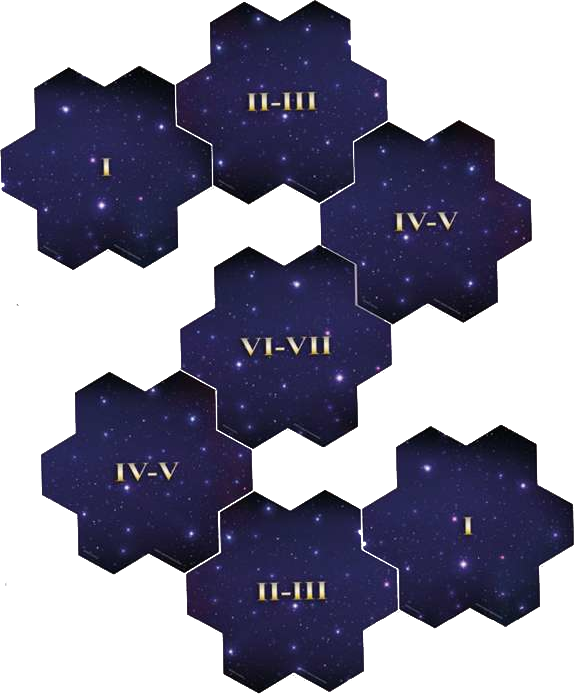
\includegraphics[width=\columnwidth, keepaspectratio]{\maps/the-hunt-2.png};
  \footnotesize{\textbf{\MakeUppercase{2-PLAYER SCENARIO}}};
\end{center}

\begin{tikzpicture}[overlay, anchor=north]
  \centering
  \node at (0, 0) {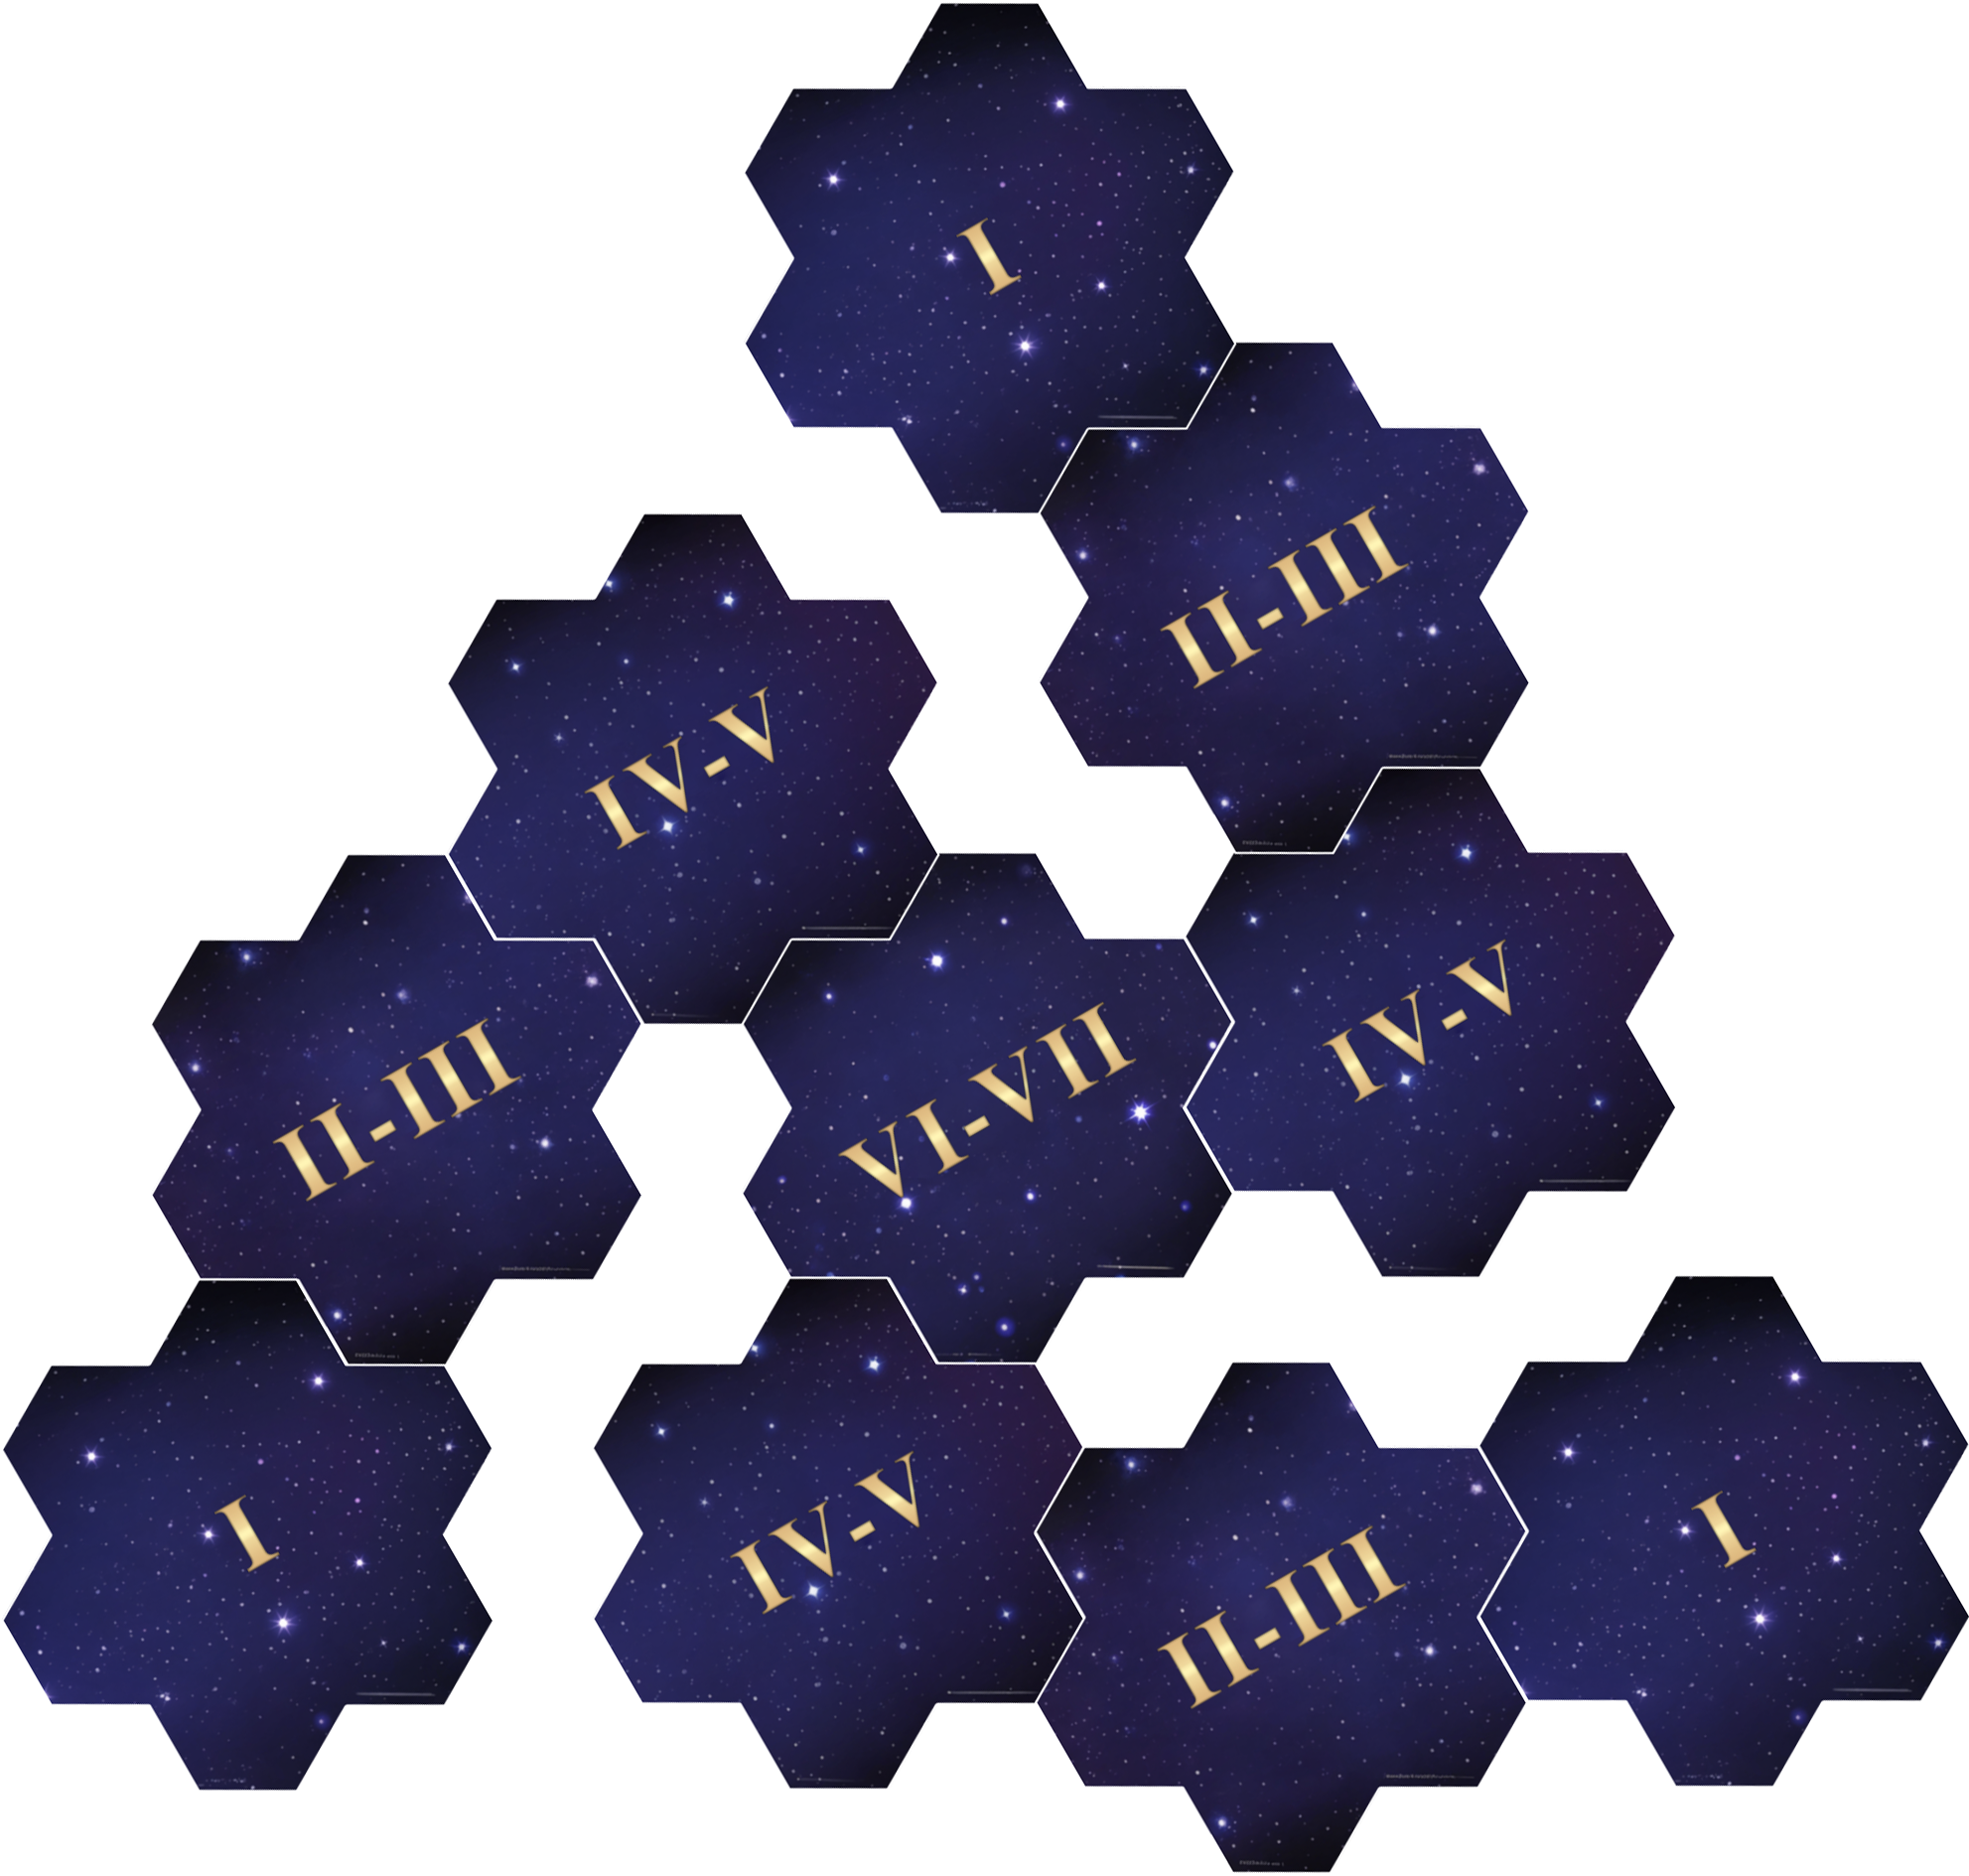
\includegraphics[width=\textwidth, height=0.48\textheight, keepaspectratio]{\maps/the-hunt-3.png}};
  \node at (0, -12) {\footnotesize{\textbf{\MakeUppercase{3-PLAYER SCENARIO}}}};
\end{tikzpicture}

\end{multicols*}

\clearpage

\begin{wrapfigure}{l}{0.3\textwidth}
  \raisebox{0pt}[\dimexpr\height-0.2\baselineskip\relax]{\framedimage[1.1\linewidth]{\art/azure_dragon.jpg}}
\end{wrapfigure}
{
  \textbf{\MakeUppercase{Boss: Azure Dragon}}

  \medskip

  \textit{Little is known of the Azure Dragon.
    It is both rare and mighty, thus few have seen it, and fewer still have survived its attacks.
    This powerful creature is not much bigger than most dragons, but is said to be capable of enduring prolonged physical attack.
    It is said those standing face-to-face with an Azure Dragon tend to freeze from pure fear.
  }

  \medskip

  \textbf{Fighting the Azure Dragon:}
  \begin{enumerate}
    \item Place the Azure Dragon Miniature/Card on the battlefield.
      Ignore its ability.
    \item Prepare a pile of discarded Artifacts and shuffle it.
  \end{enumerate}

  \medskip

  \textbf{Rules:}
  \begin{itemize}
    \item \textit{Hoarding Tendency:} At the start of each Turn, randomly choose a Card from the shuffled pile of discarded Artifacts.
      If the Artifact is:
      \begin{itemize}
        \item A weapon: The Dragon gains one Breath attack that targets three creatures in a row.
          The Unit directly hit in the middle suffers full damage, while the Units on both sides suffer 3\,\svg{damage-red} less.
        \item A piece of armor, shield, or clothing: The Dragon gains 3\,\svg{defense}, represented with spare Faction Cubes.
          Remove them after they have absorbed damage.
        \item A trinket: The Azure Dragon roars and summons an ice storm, causing all creatures to freeze in fear.
          This results in every Unit moving only 1 Field per Round, while the Azure Dragon can fly to any Field on the Combat Board.
      \end{itemize}
    \item The Azure Dragon is immune to all Spells cast against it.
    \item Buffs and enhancements cast on player's Units remain effective.
  \end{itemize}
}

\bigskip

\hommtable[]{8}{
  \centering
  \medskip

  \newcommand{\bronze}[0]{\svgunit[12]{bronze}}
  \newcommand{\silver}[0]{\svgunit[12]{silver}}
  \newcommand{\golden}[0]{\svgunit[12]{golden}}
  \newcommand{\azure}[0]{\svgunit[12]{azure}}

  \begin{tabularx}{\linewidth}{XXXX}
  \darkcell{\raisebox{-.2\height}{\svgunit[20]{bronze}} \textbf{Easy}} &
  \darkcell{\raisebox{-.2\height}{\svgunit[20]{silver}} \textbf{Normal}} &
  \darkcell{\raisebox{-.2\height}{\svgunit[20]{golden}} \textbf{Hard}} &
  \darkcell{\raisebox{-.2\height}{\svgunit[20]{azure}} \textbf{Impossible}}\\
  \lightcell[1.8]{No additional\\changes} &
  \lightcell[1.8]{\raisebox{-.25\height}{
\includegraphics[height=15px]{\images/hp.png}} 22} &
  \lightcell[1.8]{\raisebox{-.25\height}{
\includegraphics[height=15px]{\images/hp.png}} 30} &
  \lightcell[1.8]{\raisebox{-.25\height}{
\includegraphics[height=15px]{\images/hp.png}} 40 \\ +2 \svg{attack_yellow} \\ +2 \svg{defense_yellow}}
  \end{tabularx}
}

\clearpage

\begin{wrapfigure}{l}{0.3\textwidth}
  \raisebox{0pt}[\dimexpr\height-0.2\baselineskip\relax]{\framedimage[1.1\linewidth]{\art/crystal_dragon.jpg}}
\end{wrapfigure}
{
  \textbf{\MakeUppercase{Boss: Crystal Dragon}}

  \medskip

  \textit{Made entirely from red crystal and brought to life through magical means, the Crystal Dragon is literally semitransparent, lit from the center by its magical heart.
    Used frequently as a training tool for young dragon slayers, many wizards also create these creatures for the crystal they shed.
  }

  \medskip

  \textbf{Fighting the Crystal Dragon:}
  \begin{enumerate}
    \item Place the Crystal Dragon Miniature/Card on the battlefield.
      Ignore its ability.
    \item Place two Gold Golems and two Diamond Golems on the battlefield.
  \end{enumerate}

  \medskip

  \textbf{Rules:}
  \begin{itemize}
    \item At the start of every battle Round, check if any of the Golems were removed in the previous Round.
      If so, spawn one new Diamond or Gold Golem (chosen randomly) in the last row of the battlefield.
    \item \textit{Golem Devour:} The Crystal Dragon can consume Golems to regain health.
      During its Turn, if the Crystal Dragon is adjacent to a Golem, it can choose to consume it, removing a certain amount of \svg{damage-red} based on the type of Golem consumed:
      \begin{itemize}
        \item Consuming a Gold Golem: Remove 2 \svg{damage-red}.
        \item Consuming a Diamond Golem: Remove 4 \svg{damage-red}.
        \item[] \textbf{Note:} The Crystal Dragon can only consume one Golem per Turn.
      \end{itemize}
    \item Golem Abilities: Gold and Diamond Golems do not possess any additional abilities beyond those specified on their Cards.
      They primarily serve as fodder for the Crystal Dragon's health regeneration.
    \item The Crystal Dragon \textit{retaliates twice} per battle Round.
  \end{itemize}
}

\bigskip

\hommtable[]{10}{
  \centering
  \medskip

  \newcommand{\bronze}[0]{\svgunit[12]{bronze}}
  \newcommand{\silver}[0]{\svgunit[12]{silver}}
  \newcommand{\golden}[0]{\svgunit[12]{golden}}
  \newcommand{\azure}[0]{\svgunit[12]{azure}}

  \begin{tabularx}{\linewidth}{XXXX}
  \darkcell{\raisebox{-.2\height}{\svgunit[20]{bronze}} \textbf{Easy}} &
  \darkcell{\raisebox{-.2\height}{\svgunit[20]{silver}} \textbf{Normal}} &
  \darkcell{\raisebox{-.2\height}{\svgunit[20]{golden}} \textbf{Hard}} &
  \darkcell{\raisebox{-.2\height}{\svgunit[20]{azure}} \textbf{Impossible}}\\
  \lightcell[2.8]{No additional\\changes} &
  \lightcell[2.8]{\raisebox{-.25\height}{
\includegraphics[height=15px]{\images/hp.png}} 22} &
  \lightcell[2.8]{{\raisebox{-.25\height}{
\includegraphics[height=15px]{\images/hp.png}} 26 \\ +1 Retaliation}} &
  \lightcell[2.8]{\raisebox{-.25\height}{
\includegraphics[height=15px]{\images/hp.png}} 32 \\ +1 Retaliation  \\ Remove additional 2 \svg{damage-table} by consuming Golems} \\
  \end{tabularx}
}

\vspace{-2em}

\begin{wrapfigure}{l}{0.3\textwidth}
  \raisebox{0pt}[\dimexpr\height-1.2\baselineskip\relax]{\framedimage[1.1\linewidth]{\art/rust_dragon.jpg}}
\end{wrapfigure}
{
  \textbf{\MakeUppercase{Boss: Rust Dragon {\scriptsize Requires Fortress Expansion}}}

  \medskip

  \textit{Rust Dragons are known to hunt Gorgons, and live and feed in sulfur mines.
    With this appetite, Rust Dragons spew a concentrated acid as their primary attack.
    This acid is capable of eating through the strongest armor, lowering the defense of its target while inflicting further damage.
  }

  \medskip

  \textbf{Fighting the Rust Dragon:}
  \begin{enumerate}
    \item Place the Rust Dragon Miniature/Card on the battlefield.
      Ignore its ability.
    \item Prepare four spare M\&M Deck Cards to mark pools of acid.
  \end{enumerate}

  \medskip

  \textbf{Rules:}
  \begin{itemize}
    \item The Rust Dragon is immune to basic Spells.
    \item \textit{Corrosive Vomit:} The Rust Dragon has a powerful crowd control ability that allows it to spew four pools of sulfuric acid onto the battlefield \textit{at the beginning} of each Combat Round.
      Use M\&M Deck Cards placed face down to mark their locations.
    \item The Rust Dragon cannot place pools on the same Fields as in the previous Round.
      Mark the Fields with spare Faction Cubes to indicate where the pools were located.
    \item The pools of sulfuric acid block battlefield Fields and impede movement for one Round only.
      They serve as Obstacles for both players and the Dragon.
    \item The Rust Dragon's passive ability, \textit{Corrosion}, decreases an enemy Unit's armor by 2 with each attack.
      Place a spare Faction Cube on the Unit's Card to indicate this effect.
      Corrosion stacks up to -4 \svg{defense}.
  \end{itemize}
}

\vspace{5em}

\hommtable[]{9}{
  \centering
  \medskip

  \newcommand{\bronze}[0]{\svgunit[12]{bronze}}
  \newcommand{\silver}[0]{\svgunit[12]{silver}}
  \newcommand{\golden}[0]{\svgunit[12]{golden}}
  \newcommand{\azure}[0]{\svgunit[12]{azure}}

  \begin{tabularx}{\linewidth}{XXXX}
  \darkcell{\raisebox{-.2\height}{\svgunit[20]{bronze}} \textbf{Easy}} &
  \darkcell{\raisebox{-.2\height}{\svgunit[20]{silver}} \textbf{Normal}} &
  \darkcell{\raisebox{-.2\height}{\svgunit[20]{golden}} \textbf{Hard}} &
  \darkcell{\raisebox{-.2\height}{\svgunit[20]{azure}} \textbf{Impossible}}\\
  \lightcell[2.5]{No additional\\changes} &
  \lightcell[2.5]{\raisebox{-.25\height}{
\includegraphics[height=15px]{\images/hp.png}} 20} &
  \lightcell[2.5]{\raisebox{-.25\height}{
\includegraphics[height=15px]{\images/hp.png}} 32} &
  \lightcell[2.5]{\raisebox{-.25\height}{
\includegraphics[height=15px]{\images/hp.png}} 40 \\ +1 to Corrosion armor decrease} \\
  \end{tabularx}
}

\vspace{-2em}

\begin{wrapfigure}{l}{0.28\textwidth}
  \raisebox{0pt}[\dimexpr\height-0.2\baselineskip\relax]{\framedimage[1.1\linewidth]{\art/faerie_dragon.jpg}}
\end{wrapfigure}
{
  \textbf{\MakeUppercase{Boss: Faerie Dragon {\scriptsize Requires Rampart Expansion}}}

  \medskip

  \textit{Faerie Dragons are deceptively cute, but in truth, are mischievous tricksters.
    Little is known about these notorious troublemakers.
    What is known is found more in storybooks than magical tomes.
    Some say they are invisible.
    Some say they can cast spells.
    Some say Magic Mirror is one of their natural defensive traits.
  }

  \medskip

  \textbf{Fighting the Faerie Dragon:}
  \begin{enumerate}
    \item Place 2 Faerie Dragon Cards on the battlefield.
      Ignore their abilities.
    \item Place 1 Dendroid Card from the \svg{silver} Neutral Units Deck onto the battlefield, and place 3 additional Cards face down to represent the other 3 Dendroids.
  \end{enumerate}

  \medskip

  \textbf{Rules:}
  \begin{itemize}
    \item The Faerie Dragon is immune to basic Spells.
    \item The Faerie Dragon can cast up to two different Spells per battle Round.
    \item All Spells are displayed visibly next to the Combat Board:
      \begin{enumerate}
        \item The first Spell is \textit{Lightning}.
        \item The second Spell is \textit{Cure}.
        \item For the third Spell, the Faerie Dragon randomly picks an expert Spell from the Spell Deck, excluding Map \svg{map} Spells.
          If a Map \svg{map} Spell is picked, draw another Spell.
      \end{enumerate}
    \item \textit{Trickster:} In the first Round of the battle, the first targeted Faerie Dragon is a mere mirage.
      It inflicts damage, but disappears from the battlefield when hit by an enemy.
    \item Dendroids' Ability: Each Dendroid holds a key to the Faerie Dragon's power.
      After the second Dendroid dies, start removing one Spell from the Faerie Dragon's spellbook, beginning with the third Spell.
      Decrease the dragon's Spell Empowerment \svg{empower} by one (starting from its maximum) upon vanquishing the 2nd, 3rd, and 4th Dendroids.
      When there are no Dendroids left, the dragon loses the ability to cast Spells.
  \end{itemize}
}

\bigskip

\hommtable[]{7}{
  \centering
  \medskip

  \newcommand{\bronze}[0]{\svgunit[12]{bronze}}
  \newcommand{\silver}[0]{\svgunit[12]{silver}}
  \newcommand{\golden}[0]{\svgunit[12]{golden}}
  \newcommand{\azure}[0]{\svgunit[12]{azure}}

  \begin{tabularx}{\linewidth}{XXXX}
  \darkcell{\raisebox{-.2\height}{\svgunit[20]{bronze}} \textbf{Easy}} &
  \darkcell{\raisebox{-.2\height}{\svgunit[20]{silver}} \textbf{Normal}} &
  \darkcell{\raisebox{-.2\height}{\svgunit[20]{golden}} \textbf{Hard}} &
  \darkcell{\raisebox{-.2\height}{\svgunit[20]{azure}} \textbf{Impossible}}\\
  \lightcell[1.6]{No additional\\changes} &
  \lightcell[1.6]{\raisebox{-.25\height}{
\includegraphics[height=15px]{\images/hp.png}} 18} &
  \lightcell[1.6]{\raisebox{-.25\height}{
\includegraphics[height=15px]{\images/hp.png}} 26} &
  \lightcell[1.6]{\raisebox{-.25\height}{
\includegraphics[height=15px]{\images/hp.png}} 32 \\ +1 Mirage} \\
  \end{tabularx}
}
